  \section*{Part 2 : Inference in an existing Bayesian network}
 %\setcounter{page}{2}
 %\addtocounter{section}{1}
 \thispagestyle{empty}

This third lab session explores the concept of Bayesian Networks.

\subsection*{Questions}


\textit{\textbf{a) What is the risk of melt-down in the power plant during a day if no
observations have been made? What if there is icy weather?}}

\vspace{1em}

If no observation has been made, the risk of melt-down in the power plant is
equal to \textbf{0.02578}. If there is icy weather it rises to \textbf{0.03472}.

\textit{\textbf{b) Suppose that both warning sensors indicate failure. What is the risk
of a meltdown in that case? Compare this result with the risk of a melt-down
when there is an actual pump failure and water leak. What is the difference?
The answers must be expressed as conditional probabilities of the observed
variables, $P(Meltdown|...)$.}}

\vspace{1em}

$P(Meltdown| PumpFailureWar,WaterLeakWar) = 0.14535$

$P(Meltdown| PumpFailure,WaterLeak) = 0.2$

The probability of having a meltdown whent there is a pump failure and a water
leak is higher.

\textit{\textbf{c) The conditional probabilities for the stochastic variables are often
estimated by repeated experiments or observations. Why is it sometimes very
difficult to get accurate numbers for these? What conditional probabilities
in the model of the plant do you think are difficult or impossible to estimate?}}

\vspace{1em}


It is challenging to measure precisely the effect of each parameter taken separately
from the others on a given event. Furthermore some parameters are simply not
quantifiable, for example \textit{IcyWeather}. Is this relative to the temperature ?
The humidity rate? The pressure ? In this problem we have no proper definition,
therefore it is impossible to estimate.

\textit{\textbf{d) Assume that the "IcyWeather" variable is changed to a more accurate
"Temperature" variable instead (don't change your model). What are the different
 alternatives for the domain of this variable? What will happen with the
 probability distribution of P(WaterLeak | Temperature) in each alternative? }}

 \vspace{1em}

The domain will have more possible states. Instead of having simply IcyWeather true or
false based on unknown parameters, the temperature will be represented as a
number (e.g. 3°C) or as a range of temperature (e.g. 5-10°C).

%-------------------------------------------------------------------------------


\newpage
\thispagestyle{empty}

\textit{\textbf{a) What does a probability table in a Bayesian network represent?}}

\vspace{1em}

The probability table shows the probability of each possible state of a node given
the states of the parent nodes.


\textit{\textbf{b) What is a joint probability distribution? Using the chain
rule on the structure of the Bayesian network to rewrite the joint distribution
as a product of P(child|parent) expressions, calculate manually the particular
entry in the joint distribution of P(Meltdown=F, PumpFailureWarning=F,
PumpFailure=F, WaterLeakWaring=F, WaterLeak=F, IcyWeather=F).
Is this a common state for the nuclear plant to be in?}}

\vspace{1em}

The chain rule provide us with the following equation

$P(everything false) = P(IW).P(PF).P(PFW|PF).P(MD|PF, WL).P(WL|IW).P(WLW|WL)$

\hspace{9em}$= 0,95 * 0,9 * 0,95 * 1 * 0,9 * 0,95 = 0,69$

Yes this is a common state for the nuclear plant.

\textit{\textbf{c) What is the probability of a meltdown if you know that there
is both a water leak and a pump failure? Would knowing the state of any other
 variable matter? Explain your reasoning!}}

 \vspace{1em}

$P(Meltdown | PumpFailure,WaterLeak ) = 0,2$

No other variables matter.
When all the parents values are observed they alone determine the child value.


\textit{\textbf{d) Calculate manually the probability of a meltdown when you
happen to know that PumpFailureWarning=F, WaterLeak=F, WaterLeakWarning=F and
 IcyWeather=F but you are not really sure about a pump failure.}}

 \vspace{1em}

\begin{center}
The chain rule provide us with the following equation

$P(MD=T|PF unsure,else false)= P(IW).P(WL|IW).P(WLW|WL).[P(PF=T).P(PFW|PF=T).P(MD=T|PF=T,WL)+ P(PF=F).P(PFW|PF=F).P(MD=T|PF=F,WL)]$

$= 0,95*0,9*0,95*(0,1*0,1*0,2 + 0,9*0,95*0,01) = 0,008569$ (1)
\end{center}

\vspace{2em}
\begin{center}
$P(MD=F|PF unsure, else false)$

$=P(IW).P(WL|IW).P(WLW|WL)* [P(PF=T).P(PFW|PF=T).P(MD=F|PF=T,WL) + P(PF=F).P(PFW|PF=F).P(MD=F|PF=F,WL)]$

$= 0,95 * 0,9 * 0,95 * (0,1 * 0,1 * 0,80 + 0,9 * 0,95 * 0,99) =0.694027$ (2)
\vspace{2em}
$\text{(1) and (2) }=> \alpha = 1 / (0,008 + 0,69) = 1,42329 $

$(1)\text{ } 0,008 * 1,42 = 0,012\text{ and (2) }0,694 * 1,42 = 0,988 $

\end{center}



%------------------------------------------------------------------------------

\newpage
\thispagestyle{empty}
\section*{Part 3 : Extending a network}

\textit{\textbf{During the lunch break, the owner tries to show off for his
employees by demonstrating the many features of his car stereo.
To everyone's disappointment, it doesn't work. How did the owner's
chances of surviving the day change after this observation?}}

\vspace{1em}
With the assumption that the radio does not work, the probability of survival
is \textbf{$P(Survives)=0.98116$} which is less than the probability of survival without making any
observation on the radio, \textbf{$P(Survives)=0.99001$}.

\textit{\textbf{The owner buys a new bicycle that he brings to work every day.
How does the bicycle change the owner's chances of survival?}}

\vspace{1em}
With the addition of the bicycle to the network, the probability of survival
increases slightly $P(Survives)=0.99505$.

\textit{\textbf{It is possible to model any function in propositional
logic with Bayesian Networks. What does this fact say about the complexity
of exact inference in Bayesian Networks? What alternatives are there
to exact inference?}}



\newpage
\thispagestyle{empty}
\section*{Part 4 : More extensions}

\begin{figure}[h]
    \centering
      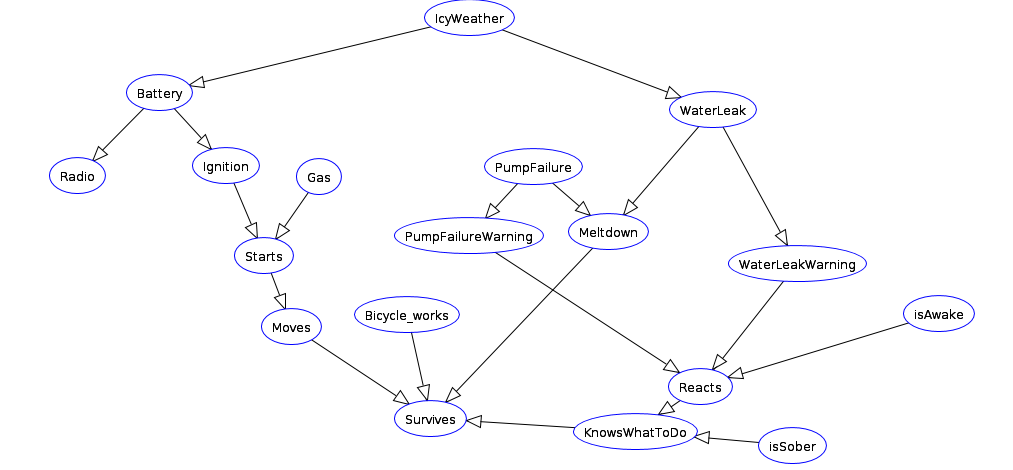
\includegraphics[width=0.83\linewidth]{./images/lab3.png}
    \caption{Adding Mr H.S.\label{graph}}
\end{figure}

With the addition of Mr H.S. to the network, the probability of survival
increases slightly $P(Survives)=0.99522$.

With the observation of Meltdown and Reacts, $P(Survives)=0.82104$.

\textit{\textbf{The owner had an idea that instead of employing a safety person,
to replace the pump with a better one. Is it possible, in your model, to
compensate for the lack of Mr H.S.'s expertise with a better pump?}}

\vspace{1em}
Without Mr H.S. it is possible to achieve the same probability of survival by
decreasing the probability of PumpFailure by only 1%.

\textit{\textbf{Mr H.S. fell asleep on one of the plant's couches.
 When he wakes up he hears someone scream: "There is one or more warning
 signals beeping in your control room!". Mr H.S. realizes that he does not
 have time to fix the error before it is to late (we can assume that he wasn't
  in the control room at all). What is the chance of survival for Mr H.S. if he
   has a car with the same properties as the owner? Hint: This question involves
    a disjunction (A or B) which can not be answered by querying the network
    as is. How could you answer such questions? Maybe something could be added
    or modified in the network.}}

\textit{\textbf{What unrealistic assumptions do you make when creating a
Bayesian Network model of a person?}}

\vspace{1em}
We make the assumption that human actions are predictable. Furthermore, we do not
consider the gain of experience which would modify the probabilities, for exemple
Mr H.S. will be less incompetent.

\textit{\textbf{Describe how you would model a more dynamic world where for
 example the "IcyWeather" is more likely to be true the next day if it was
 true the day before. You only have to consider a limited sequence of days.}}

 \vspace{1em}
We would have to add nodes representing the weather of the previous days.
The node representing the previous day should have more impact on IcyWeather that
the day before and so on until the last weather saved.

\newpage
\thispagestyle{empty}
